%% 
%% Copyright 2007-2024 Elsevier Ltd
%% 
%% This file is part of the 'Elsarticle Bundle'.
%% ---------------------------------------------
%%  
%% It may be distributed under the conditions of the LaTeX Project Public
%% License, either version 1.3 of this license or (at your option) any%% later version.  The latest version of this license is in
%%    http://www.latex-project.org/lppl.txt
%% and version 1.3 or later is part of all distributions of LaTeX
%% version 1999/12/01 or later.
%% 
%% The list of all files belonging to the 'Elsarticle Bundle' is
 %% given in the file `manifest.txt'.
%% 
%% Template article for Elsevier's document class `elsarticle'
%% with harvard style bibliographic references

\documentclass[preprint,12pt,authoryear]{elsarticle}

%% Use the option review to obtain double line spacing
%% \documentclass[authoryear,preprint,review,12pt]{elsarticle}

%% Use the options 1p,twocolumn; 3p; 3p,twocolumn; 5p; or 5p,twocolumn
%% for a journal layout:
%% \documentclass[final,1p,times,authoryear]{elsarticle}
%% \documentclass[final,1p,times,twocolumn,authoryear]{elsarticle}
%% \documentclass[final,3p,times,authoryear]{elsarticle}
%% \documentclass[final,3p,times,twocolumn,authoryear]{elsarticle}
%% \documentclass[final,5p,times,authoryear]{elsarticle}
%% \documentclass[final,5p,times,twocolumn,authoryear]{elsarticle}

%% For including figures, graphicx.sty has been loaded in
%% elsarticle.cls. If you prefer to use the old commands
%% please give \usepackage{epsfig}

%% The amssymb package provides various useful mathematical symbols
\usepackage{amssymb}
\usepackage{graphicx}
%% The amsmath package provides various useful equation environments.
\usepackage{amsmath}
\usepackage{algorithm}
\usepackage{algorithmicx}
\usepackage{algpseudocode}
%% The amsthm package provides extended theorem environments
%% \usepackage{amsthm}

%% The lineno packages adds line numbers. Start line numbering with
%% \begin{linenumbers}, end it with \end{linenumbers}. Or switch it on
%% for the whole article with \linenumbers.
%% \usepackage{lineno}

\journal{Computers and Operation Research}

\begin{document}

\begin{frontmatter}

%% Title, authors and addresses

%% use the tnoteref command within \title for footnotes;
%% use the tnotetext command for theassociated footnote;
%% use the fnref command within \author or \affiliation for footnotes;
%% use the fntext command for theassociated footnote;
%% use the corref command within \author for corresponding author footnotes;
%% use the cortext command for theassociated footnote;
%% use the ead command for the email address,
%% and the form \ead[url] for the home page:
%% \title{Title\tnoteref{label1}}
%% \tnotetext[label1]{}
%% \author{Name\corref{cor1}\fnref{label2}}
%% \ead{email address}
%% \ead[url]{home page}
%% \fntext[label2]{}
%% \cortext[cor1]{}
%% \affiliation{organization={},
%%            addressline={}, 
%%            city={},
%%            postcode={}, 
%%            state={},
%%            country={}}
%% \fntext[label3]{}

\title{Actor-based Large Neighborhood Search for weekly maintenance scheduling} %% Article title

%% use optional labels to link authors explicitly to addresses:
%% \author[label1,label2]{}
%% \affiliation[label1]{organization={},
%%             addressline={},
%%             city={},
%%             postcode={},
%%             state={},
%%             country={}}
%%
%% \affiliation[label2]{organization={},
%%             addressline={},
%%             city={},
%%             postcode={},
%%             state={},
%%             country={}}

\author{Christian Brunbjerg Jespersen} %% Author name
\author{Kristoffer Sigsgaard Wernblad}
\author{Thomas Jacob Riis Stidsen}
\author{Kasper Barslund Hansen}
\author{Jingrui Ge}
\author{Simon Didriksen}
\author{Niels Henrik Mortensen}

%% Author affiliation
\affiliation{organization={Technical University of Denmark},%Department and Organization
            addressline={Anker Egelundsvej 1}, 
            city={Kongens Lyngby},
            postcode={2800}, 
            state={Hovedstaden},
            country={Denmark}}
\affiliation{organization={Technical University of Denmark},%Department and Organization
            addressline={Anker Egelundsvej 1}, 
            city={Kongens Lyngby},
            postcode={2800}, 
            state={Hovedstaden},
            country={Denmark}}
\affiliation{organization={Technical University of Denmark},%Department and Organization
            addressline={Anker Egelundsvej 1}, 
            city={Kongens Lyngby},
            postcode={2800}, 
            state={Hovedstaden},
            country={Denmark}}
\affiliation{organization={Technical University of Denmark},%Department and Organization
            addressline={Anker Egelundsvej 1}, 
            city={Kongens Lyngby},
            postcode={2800}, 
            state={Hovedstaden},
            country={Denmark}}
\affiliation{organization={Technical University of Denmark},%Department and Organization
            addressline={Anker Egelundsvej 1}, 
            city={Kongens Lyngby},
            postcode={2800}, 
            state={Hovedstaden},
            country={Denmark}}
\affiliation{organization={Technical University of Denmark},%Department and Organization
            addressline={Anker Egelundsvej 1}, 
            city={Kongens Lyngby},
            postcode={2800}, 
            state={Hovedstaden},
            country={Denmark}}
\affiliation{organization={Technical University of Denmark},%Department and Organization
            addressline={Anker Egelundsvej 1}, 
            city={Kongens Lyngby},
            postcode={2800}, 
            state={Hovedstaden},
            country={Denmark}}
%% Abstract
\begin{abstract}
%% Text of abstract
Many planning problems facing the operations research field have proven difficult to solve due to their inherent uncertainty and highly dynamic nature. Stochastic optimization~\citep{???}, fuzzy logic~\citep{???}, and robust optimization~\citep{???} are some of the methods that have been proposed to solve these issues. These methods make an implicit assumption of a static data setting and a static problem setting. Maintenance scheduling is one such problem where the best available information continually updates and then therefore the scheduling continuously needs to be updated. Maintenance scheduling is a complex process often more associated with operation management, but here we will argue that is possible to implement general maintenance scheduling approaches, if the solution approach is designed to be integrated into a business
process of the kind that are usually developed by the principles of operation management. 

This paper proposes a novel optimization method that is capable to optimizing a scheduling problem in the following setting:  Primary data source is changing in real-time; external inputs affects the optimization process; multiple actors are making interdependent decision whose objectives may differ significantly. The proposed solution approach is an actor-based framework including a large neighborhood search metaheuristic implementation. The framework is tested on the real-world problem of maintaining scheduling of oil platforms for Total in the North Sea, but the approach is very general and can be applied to a wide variety of other planning problems.
\end{abstract}

%%Graphical abstract
%\begin{graphicalabstract}
%\includegraphics{grabs}
%\end{graphicalabstract}

%%Research highlights
%\begin{highlights}
%\item How to allow direct and real-time integration into an optimization process?
%\item How to perform optimization in a real-time changing parameter space?
%\end{highlights}

%% Keywords
\begin{keyword}
%% keywords here, in the form: keyword \sep keyword
Large Neighborhood Search \sep Actor Framework \sep Maintenance scheduling \sep Real-time Optimization \sep Human-centered Computing \sep Interactive Systems and Tools \sep Decision Support Systems \sep Interactive Optimization.


%% PACS codes here, in the form: \PACS code \sep code

%% MSC codes here, in the form: \MSC code \sep code
%% or \MSC[2008] code \sep code (2000 is the default)

\end{keyword}

\end{frontmatter}

%% Add \usepackage{lineno} before \begin{document} and uncomment 
%% following line to enable line numbers
%% \linenumbers

%% main text
%%

%% Use \section commands to start a section
\section{Introduction}
\label{sec:1-introduction}
%% Labels are used to cross-reference an item using \ref command.

Maintenance scheduling is an operational problem that have proven hard to solve (NP-hard~\cite{???}). Furthermore, for optimization to be utilized the dynamic and uncertain nature of maintenance scheduling requires a tight integration with third party administration software to enable the tacit knowledge of decision makers to influence the planning process easily. Often a number of different decision makers at different company levels take part in the planning process and in this way the industry usually assigns responsibility for decision-making  to an individual representing only a small part of the complete process. 

These multiple smaller planning processes are often difficult to map to a single mathematical model describing the whole system as elaborated by (\citep{barthelemy_human_2002}). Solving operation research problems that are operational in nature have additional requirements over conventional static problems: they have to be responsive to changing parameters; able to be assimilated into the decision-makers workflow; allow for integration with dynamic data sources such as databases and RESTapi \citep{meignan_review_2015}. Operational aspects of operation research, as opposed to higher level strategic and tactical aspects, are characterized by extensive amounts negotiation and feedback on proposed schedules. The lack of integration and responsiveness can lead to schedules that are not directly implemented in practice but instead provides initial suggestions \cite{meignan_review_2015}, which are then iterated else where in the scheduling process. In \citep{barthelemy_human_2002} the authors argue that many problems that operation research aim to solve are often composed of a group of individuals whose decisions are consolidated into an "epistemic subject" for which a mathematical model can be formulated and solved, with many scheduling problems being good examples. However often multiple actors have different views on what constitutes an optimal schedule hence resulting in multiple-objectives. Even if multi-objective optimization~\citep{???} is applied to find the Pareto Front~\citep{???} a negotiating process still is needed between the actors to select the final schedule.

This paper proposes a solution method that will allow for real-time optimization based on actor/user interaction and connection to a dynamic data source, effectively managing the changes to the parameter space. The proposed solution method will be tested on the multi-compartment multi-knapsack problem (MCMKP) for maintenance scheduling on a large dataset from a company. The MCMKP naturally models what in the practical maintenance is called the weekly schedule, taken form \citep{palmerMaintenancePlanningScheduling2019}. It should be noted that the scientific maintenance scheduling literature deviates significantly from its practical implementation which is detailed in \citep{palmerMaintenancePlanningScheduling2019}. The solution method will by based on the large neighborhood search (LNS) metaheuristic. This meta heuristic was chosen due to its properties of naturally being able to work with and fix infeasible solutions and its state of the art performance on various scheduling problems. 

To understand the need for actor-based methods some background knowledge will be required about the maintenance scheduling process. In figure \ref{fig:simple-maintenance-process} illustrates the general setup of a healthy maintenance planning and scheduling system. The systems actors have the following responsibilities: the planner generates the work orders that are to be scheduled; the scheduler creates weekly schedules based on a knapsack formulation; based on the weekly schedule the supervisor assigns work order activities that the work order is composed of (the assignment problem); the technicians executes the work in sequential pattern (single machine scheduling). A final point on the necessity of actor-based approaches to model should a setup is the idea of ownership of a work order. Throughout the scheduling process a work order is owned by a specific actor and he alone is allow to modify it. This means that a single model approach is very difficult to implement in practice as a work order looks different depending on the actor that currently owns it. This also highlight another an point in maintenance scheduling: that the stochastic nature of the maintenance scheduling process can be handled using a change of model each with different levels of aggregation, opposed to more academic approaches such as fuzzy logic and stochastic optimization.

When the fundamental uncertainties manifest themselves during planning or execution work orders are rescheduled by moving between the different actor (models), meaning that the stochastic elements of maintenance scheduling are handled by dynamic rescheduling between the actors.

\begin{figure}

\includegraphics[width=1.0\textwidth]{figures/Scheduling Process Simple.png}
\caption{Simple overview of the scheduling process with its primary types of actors. The planner, the scheduler, the supervisor(s), and the technicians. The green color highlights the scheduler as it the actor in the maintenance scheduling process that is the foundation for the paper.}
\label{fig:simple-maintenance-process}
\end{figure}

This article describes a number of contributions: 

\begin{itemize}
\item A novel actor/optimization framework
\item A novel specialized (A)LNS metaheuristic, to be utilized in an actor framework
\item Implementation and test on a large realworld maintenance scheduling problem
\end{itemize}

The paper is divided into four different sections. Section \ref{sec:2-solution-method} explains the weekly maintenance scheduling model in detail and forms the fundation of the paper. Section \ref{sec:3-results} shows that results coming from the implemented system where the implementation will be affected by simulated user-interaction. Section \ref{sec:4-discussion} will discuss the implications of the research and possible future research directions.

\subsection{A generic maintenance scheduling model}
\label{sub2sec2}
A large company needs to create a weekly maintenance plan for the next $p \in P$ weeks. The maintenance plan is planned centrally and consists of scheduling the $w \in W$ work orders, i.e. maintenance tasks, such that all are scheduled into different weeks. Each work order requires some resourses to be carried out, e.g. man-power with different qualifications, equipment etc. all of these resourses are available in limited amounts and are called traits $\tau \in T$. To simplify matters, we will assume that the recourse limits are not hard but extra workers can be paid overtime, extra equipment can be rented etc., at the cost (penalty) of $pen_{p\tau}$. The urgency of the different maintenance operations varies and is reflected in a penalty for carrying out a maintenance work order in a certain week $v_{wp}(t)$. Urgent tasks have quickly increasing penalties for the later weeks week $p$. Furthermore, two sets exists which will either will require the work order to be carried out in week $p$, i.e. $(w,p) \in E$ and a set which forbids a work order to carried out in week $p$, i.e. $(w,p) \in I$. The model for the problem is the Multi-compartment Multi-knapsack Problem with capacity penalties MCMKP.

The notation used in the model is based on the notation from the dynamic metaheuristics literature as found in \cite{yangMetaheuristicsDynamicCombinatorial2013}, where $t$ is added as a time variable on all sets, parameters, and variables that are subject to change.
This allows us to be precise in the timing on the messages that are send to the Ab-LNS.  

%\subsection{The Weekly Schedule: Multi-compartment Multi-knapsack Problem with capacity penalties}
%\label{sub2sec2}
%The actor-based large neighborhood search is implemented on the MCMKP which models that weekly schedule in maintenance. The model is comprised of five different sets. $P$ is the number of weekly periods; $W$ is the number of work orders; $\tau$ is the number of different traits; $E$ is a set that defines which work orders should be excluded from a specific weekly period; $I$ is an inclusion set that defines the allocation of specific work orders which should be included in a specific weekly period. The model has four parameters. $v_{pw}$ is the value of work order $w$ in weekly period $p$; $d$ is the penalty for exceeding a specific trait capacity; $c_{w\tau}$ is the capacity requirement for work order $w$ for trait $t$; $cap_{p\tau}$ is the total amount of capacity available in for weekly period p for for trait t. The model has 2 decision variables. $x_{wp}$, is a binary decision variable equal to one if work order w is in weekly period p and zero otherwise; $pen_{p\tau}$ is non-negative decision variable equal to the amount of excess capacity above the $cap_{p\tau}$ in weekly period p for trait $\tau$. The parameters $v$, $cap$, $Q$, and $P$ are functions of time, $\tau$, in this case as they will be subject to change during the solution process.

\include{../../tex/models/strategic}
% \begin{alignat}{2}
% 	& \text{Min} \quad \sum_{w = 1}^{W} \sum_{p = 1}^{P} v_{wp}(t) \cdot x_{wp}(t) + \sum_{p = 1}^{P} \sum_{\tau = 1}^T d \cdot pen_{p\tau}(t)   \label{eqn:objective_function_strategic} \\[1em]
%     & \text{subject to:} \notag                                                                                                                                        \\[1em]
% 	& \sum_{w = 1}^W c_{w\tau} \cdot x_{wp}(t) \leq \ cap_{p\tau}(t) + pen_{p\tau}(t)        && \forall p \in P, \forall \tau \in T                      \label{eqn:capacity_constraint}          \\[1em]
% 	& \sum_{w = 1}^{W} x_{wp}(t) = 1                                            && \forall p \in P                                       \label{eqn:single_workorder_constraint}  \\[1em]
% 	& x_{wp}(t) = 0                                                             && \forall (w, p) \in E(t)                               \label{eqn:exclusion_constraint}         \\[1em]
% 	& x_{wp}(t) = 1                                                             && \forall (w, p) \in I(t)                               \label{eqn:inclusion_constraint}         \\[1em]
% 	& x_{wp}(t) \in \{0, 1\}                                                    && \forall w \in W, \forall p \in P                      \label{eqn:x_integrality_constraint}     \\[1em] 
% 	& pen_{p\tau}(t) \in \mathbb{R}^{+}                                         && \forall p \in P, \forall \tau \in T                      \label{eqn:p_non_negativity_constraint}
% \end{alignat}

The objective function \eqref{eqn:objective_function_strategic} minimizes the total weight of all work order assignments together with the penalty $d$ for exceeding the capacity given in constraint \eqref{eqn:capacity_constraint}. Constraint \eqref{eqn:capacity_constraint} ensures that all the weights $c_{w\tau}$ for each activity in an work order, given that it has been assigned, is lower than the capacity for each period and for each trait $\tau$. $pen_{p\tau}$ is the amount of exceeded capacity that is needed for the current assignment of work order to be feasible. Constraint \eqref{eqn:single_workorder_constraint} makes sure that each work order is assigned to at least a single period. Constraint \eqref{eqn:exclusion_constraint} excludes a work order from a certain period and constraint \eqref{eqn:inclusion_constraint} forces a specific work order to be in a specific period. Constraint \eqref{eqn:x_integrality_constraint} and \eqref{eqn:p_non_negativity_constraint} specify the variable domain for $x_{wp}$ and $pen_{p\tau}$ respectively. The effects of changing $E$, $I$, $cap$, and $v$ in real-time will be examined to determine their effects on the weekly schedules and objective value.

\section{Solution Method}
\label{sec:2-solution-method}

\subsection{Actor-based Large Neighborhood Search}
A problem which is affected by user-interaction and requires real-time feedback needs an optimization approach that is able to repair infeasible schedules and while also 
converging quickly. For this the large neighborhood search metaheuristic has been shown satisfy these requirements in the literature \cite{gendreauHandbookMetaheuristics2019}. 

The LNS metaheuristic is defined for static problems, meaning that the parameters that make up the problem instance is not subject to change 
after the algorithm has been started. To make the LNS able adapt to changing parameters in real-time a message system have been implemented into the existing framework. This 
extension is shown in algorithm \ref{algo1}.  

\subsubsection{Messages And Destructors}
LNS in its most basic form has one constructor and one destructor which repeatedly destroy and rebuild the schedule. For the AbLNS we will generalize on this concept by 
including messages as destructors of the classic LNS implementation. This generalization can be seen as being somewhat similar to how the adaptive LNS (ALNS) is formulated,
but where the different constructors and destructors are chosen externally as well. 

Extending on the classic setup we define the following set of destructors, $M$:

\begin{itemize}
	\item $m_1$: Inclusion destruct message	
	\item $m_2$: Exclusion destruct message	
	\item $m_3$: Capacities destruct message	
	\item $m_4$: Weights destruct message	
	\item $m_5$: Random destruct message
\end{itemize}

Each of these messages affect different parts of the MCMK problem (weekly schedule). Notice
here that the first four messages destruct the solution by changing the parameter space and the last message is 
a random destructor.

Generalizing the destructors from being static structures into messages
allows the solution to change in real-time to a changing paramenter space meaning
that the algorithm does not need to restart to handle changes in data. 

\include{../../tex/algorithms/actor-based-large-neighborhood-search}
% \begin{algorithm}[H]
% \caption{Actor-based Large Neighborhood Search}  \label{algo1}
% \begin{algorithmic}[1]
% \State \textbf{Input} queue = message queue
% \State \textbf{Input} P     = problem instance
% \State \textbf{Input} x     = initial schedule
% % \State $x^b = x$
% \While{true}
% 	\While{queue.has\_message()}
%         % \State $m = queue.pop()$
%         % \State $m.destruct(x^b)$
% 		\State $P.update(m)$
%         \State $x.destruct(m)$
%     \EndWhile
	
%     \State $x^t = x.repair()$
%     % \If{accept($x^t$,\ $x$)}                       \label{alg:acceptance_criteria_start}
%     %     \State x = x$^t$
%     % \EndIf                                         \label{alg:acceptance_criteria_end}
%     \If{$c(x^t) < c(x)$}                             \label{alg:objective_start}
%         \State $x = x^t$
% 		\State queue.send($x$)
%     \EndIf                                           \label{alg:objective_end}
% 	\State queue.push($m_5$)
% \EndWhile\\
% \Return $x^b$
% \end{algorithmic}
% \end{algorithm}

The basic LNS setup have here been extended with a `message queue`. This message queue will be read from on every iteration of the LNS's main iteration loop. Here we notice that the 
incoming message is able to change both the solution but also the problem instance itself. Here we see one of the defining features of the LNS metaheuristic in play, that due to its inherent 
property of being able to optimize a solution that have become infeasible which is something that is very likely to happen when you change the parameter of the problem instance itself. 

Another less obvious property the message queue allows is for the algorithm to run indefinitely and instead of restarting the algorithm you instead pass 
messages to it to allow it be adjust both the solution space and the parameter space.
This property avoid the issue of time consuming initial convergence as the algorithm will be found in an optimimal state when the solution is perturbed.  

\section{Results}
\label{sec:3-results}
The results section will: 1. introduce the real-world data instance; 2. show the effect of forcing item set in the specific weekly schedules; 3. show the effect of changing the 
period capacities, and 4. show the effect of dynamically changing the value of the work orders $v$. 

\subsection{Data Instance}
\begin{table}[H]
\centering
\begin{tabular}{|c|c|c|c|c|}
\hline
           & \begin{tabular}[c]{@{}c@{}}Number of\\ Item Sets\end{tabular} & \begin{tabular}[c]{@{}c@{}}Number of\\ Compartments\end{tabular} & \begin{tabular}[c]{@{}c@{}}Number of\\ Knapsacks\end{tabular} \\ \hline
Instance 1 & 3487                                                          & 16                                                               & 52                                                            \\ \hline
\end{tabular}

\caption{Table Caption} % \label{fig1}
\end{table}
% \begin{table}[t]%% placement specifier
% %% Use tabular environment to tag the tabular data.
% %% https://en.wikibooks.org/wiki/LaTeX/Tables#The_tabular_environment
% \centering%% For centre alignment of tabular.
% \begin{tabular}{l c r}%% Table column specifiers
% %% Tabular cells are separated by &
%   1 & 2 & 3 \\ %% A tabular row ends with \\
%   4 & 5 & 6 \\
%   7 & 8 & 9 \\
% \end{tabular}
% %% Use \caption command for table caption and label.
% \end{table}

\subsection{Response to Inclusion}
The response to the inclusion of a work order is given by I parameter of the model which 
is constrained in \ref{eqn:inclusion_constraint} of model given in \ref{sub1sec2}.

The inclusion is made of forcing certain allocations of work orders to be in specific periods. Below a table is provided 
to show what changes will occur and at what and at what point in time.
\begin{table}[H]
\centering
\begin{tabular}{|c|c|c|c|c|c|}
\hline
\begin{tabular}[c]{@{}c@{}}\end{tabular}     & \begin{tabular}[c]{@{}c@{}}At Time:\\ 01:00\end{tabular} & \begin{tabular}[c]{@{}c@{}}At Time:\\ 02:00\end{tabular} & \begin{tabular}[c]{@{}c@{}}At Time:\\ 03:00\end{tabular} & \begin{tabular}[c]{@{}c@{}}At Time:\\ 04:00\end{tabular} & \begin{tabular}[c]{@{}c@{}}At Time:\\ 05:00\end{tabular} \\ \hline
\begin{tabular}[c]{@{}c@{}}$\Delta |P|$\end{tabular} & 10                                                       & 20                                                       & 30                                                       & 40                                                       & 50                                                       \\ \hline
\end{tabular}
\end{table}

With the inputs defined we will explain the main results which are shown in the figure below. 
% Use figure environment to create figures
% Refer following link for more details.
% https://en.wikibooks.org/wiki/LaTeX/Floats,_Figures_and_Captions
\begin{figure}[H]%% placement specifier
%% Use \includegraphics command to insert graphic files. Place graphics files in 
%% working directory.
\centering%% For centre alignment of image.
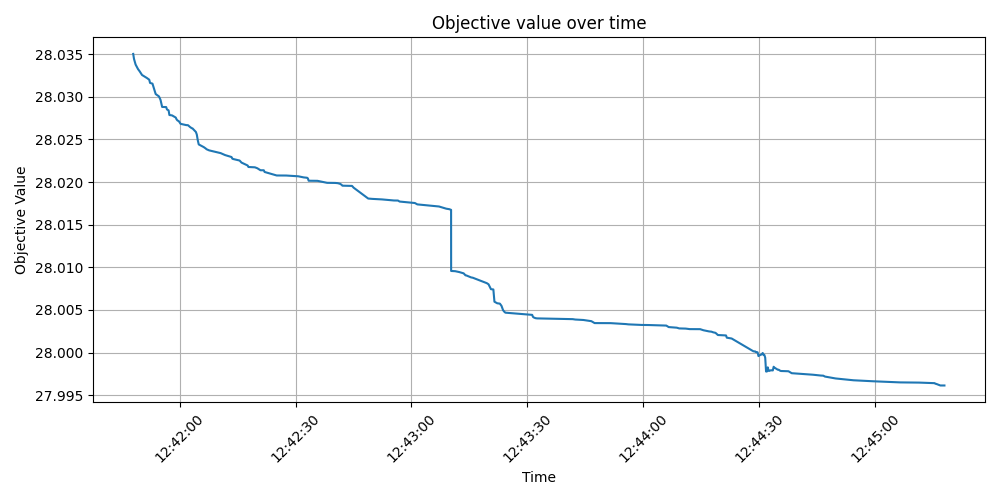
\includegraphics[width=1.0\textwidth]{figures/objective.png}
%% Use \caption command for figure caption and label.
\caption{Figure Caption}\label{fig:response-to-inclusion}
%% https://en.wikibooks.org/wiki/LaTeX/Importing_Graphics#Importing_external_graphics
\end{figure}

\subsection{Response to Exclusion}
\begin{figure}[H]%% placement specifier
%% Use \includegraphics command to insert graphic files. Place graphics files in 
%% working directory.
\centering%% For centre alignment of image.
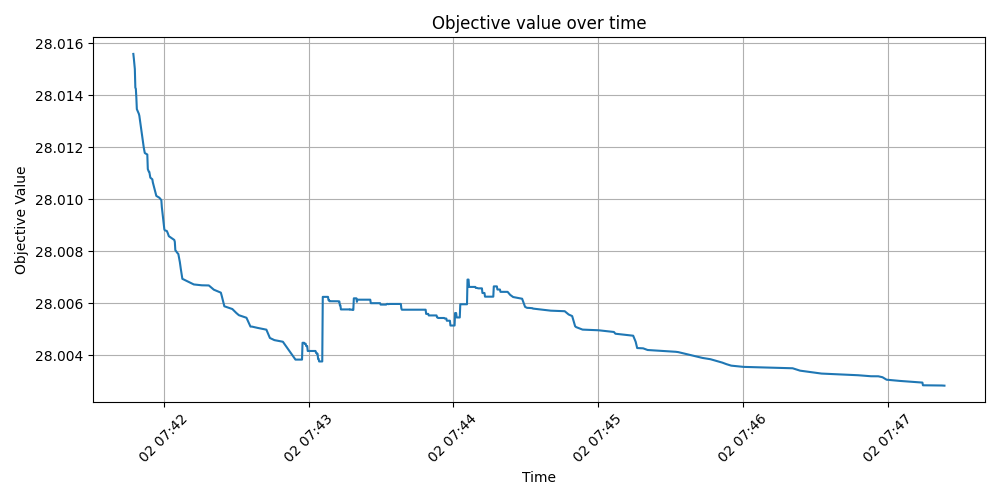
\includegraphics[width=1.0\textwidth]{figures/objective-400-exclusions.png}
%% Use \caption command for figure caption and label.
\caption{Figure Caption}\label{fig:objective-exclusion-400}
%% https://en.wikibooks.org/wiki/LaTeX/Importing_Graphics#Importing_external_graphics
\end{figure}

\subsection{Response to Changes in Knapsack Capacities}
The effects of changes to capacities will be illustrated in the same way as it was with the response to inclusion and below we see the table that shows which inputs that the AbLNS will be affected by.

\begin{table}[H]
\centering
\begin{tabular}{|c|c|c|c|c|c|}
\hline
                      & \begin{tabular}[c]{@{}c@{}}At Time:\\ 01:00\end{tabular} & \begin{tabular}[c]{@{}c@{}}At Time:\\ 02:00\end{tabular} & \begin{tabular}[c]{@{}c@{}}At Time:\\ 03:00\end{tabular} & \begin{tabular}[c]{@{}c@{}}At Time:\\ 04:00\end{tabular} & \begin{tabular}[c]{@{}c@{}}At Time:\\ 05:00\end{tabular} \\ \hline
$\Delta |p|$ & 16                                                       & 16                                                       & 16                                                       & 16                                                       & 16                                                       \\ \hline
$\Delta |\tau|$ & 16                                                       & 16                                                       & 16                                                       & 16                                                       & 16                                                       \\ \hline
$\Delta |cap|$& 100                                                      & 200                                                      & 400                                                      & 800                                                      & 1600                                                     \\ \hline
\end{tabular}
\end{table}

\begin{figure}[H]%% placement specifier
%% Use \includegraphics command to insert graphic files. Place graphics files in 
%% working directory.
\centering%% For centre alignment of image.
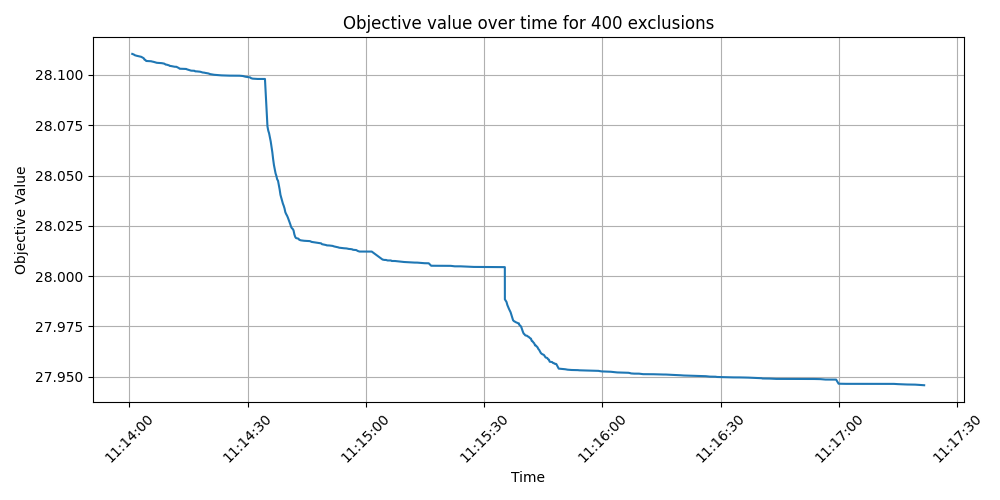
\includegraphics[width=1.0\textwidth]{figures/objective-resource-increases.png}
%% Use \caption command for figure caption and label.
\caption{Figure Caption}\label{fig:objective-resource-increases}
%% https://en.wikibooks.org/wiki/LaTeX/Importing_Graphics#Importing_external_graphics
\end{figure}

Correspondingly we also have the figure below in which the resources are decreasing.

\subsection{Response to Changes in Item Weights}
The final parameter that will be changed is the work order value $v$. This section will be more elaborate as we have to show how that the
work orders are rearranged due to the changes in their value across the different periods.

\begin{table}[H]
\centering
\begin{tabular}{|c|c|c|c|c|c|}
\hline
             & \begin{tabular}[c]{@{}c@{}}At Time:\\ 01:00\end{tabular} & \begin{tabular}[c]{@{}c@{}}At Time:\\ 02:00\end{tabular} & \begin{tabular}[c]{@{}c@{}}At Time:\\ 03:00\end{tabular} & \begin{tabular}[c]{@{}c@{}}At Time:\\ 04:00\end{tabular} & \begin{tabular}[c]{@{}c@{}}At Time:\\ 05:00\end{tabular} \\ \hline
$\Delta |w|$ & 20                                                       & 40                                                       & 80                                                       & 160                                                      & 320                                                      \\ \hline
$\Delta |p|$ & 26                                                       & 26                                                       & 26                                                       & 26                                                       & 26                                                       \\ \hline
$\Delta |v|$ & $1 \cdot 10^{5}$                                         & $2 \cdot 10^{5}$                                         & $4 \cdot 10^{5}$                                         & $8 \cdot 10^{5}$                                         & $1.6 \cdot 10^{6}$                                       \\ \hline
\end{tabular}
\end{table}

\section{Discussion}
\label{sec:4-discussion}

Maintenance scheduling efficiently solves a complex scheduling problem by the use of multiple actors. Through the use of actors the 
process handles uncertainty that is difficult to reason about, using models with different levels of aggregation where each actors understands
how to exploit his model. As uncertainties manifest themselves the actors/models handle the uncertainty through 
communication. To further understand the implications of the approach the discussion will be divided into three sections: 1. actors and 
integration; 2. continuous optimization allows asynchronous optimization; 3. future research.

\subsection{Actors \& Integration}
Often in operation research the failure to reliably solve industry problems are not due to the problems being computationally intractable 
but more a practical problem of connecting data streams so that the solution approach is connected to dynamic data source of the company
and then connecting the solution approach(s) to the relevant stakeholder (actors) through a relevant interface. The actor-based approach 
proposed in this paper makes integration easier by naturally encapsulation a model with a reliable interface. To better understand the 
novel properties of this consider the extension of figure 

\ref{fig:simple-maintenance-process}

as shown in figure \ref{fig:integrated:maintenance-process}.


\begin{figure}[H]
\centering
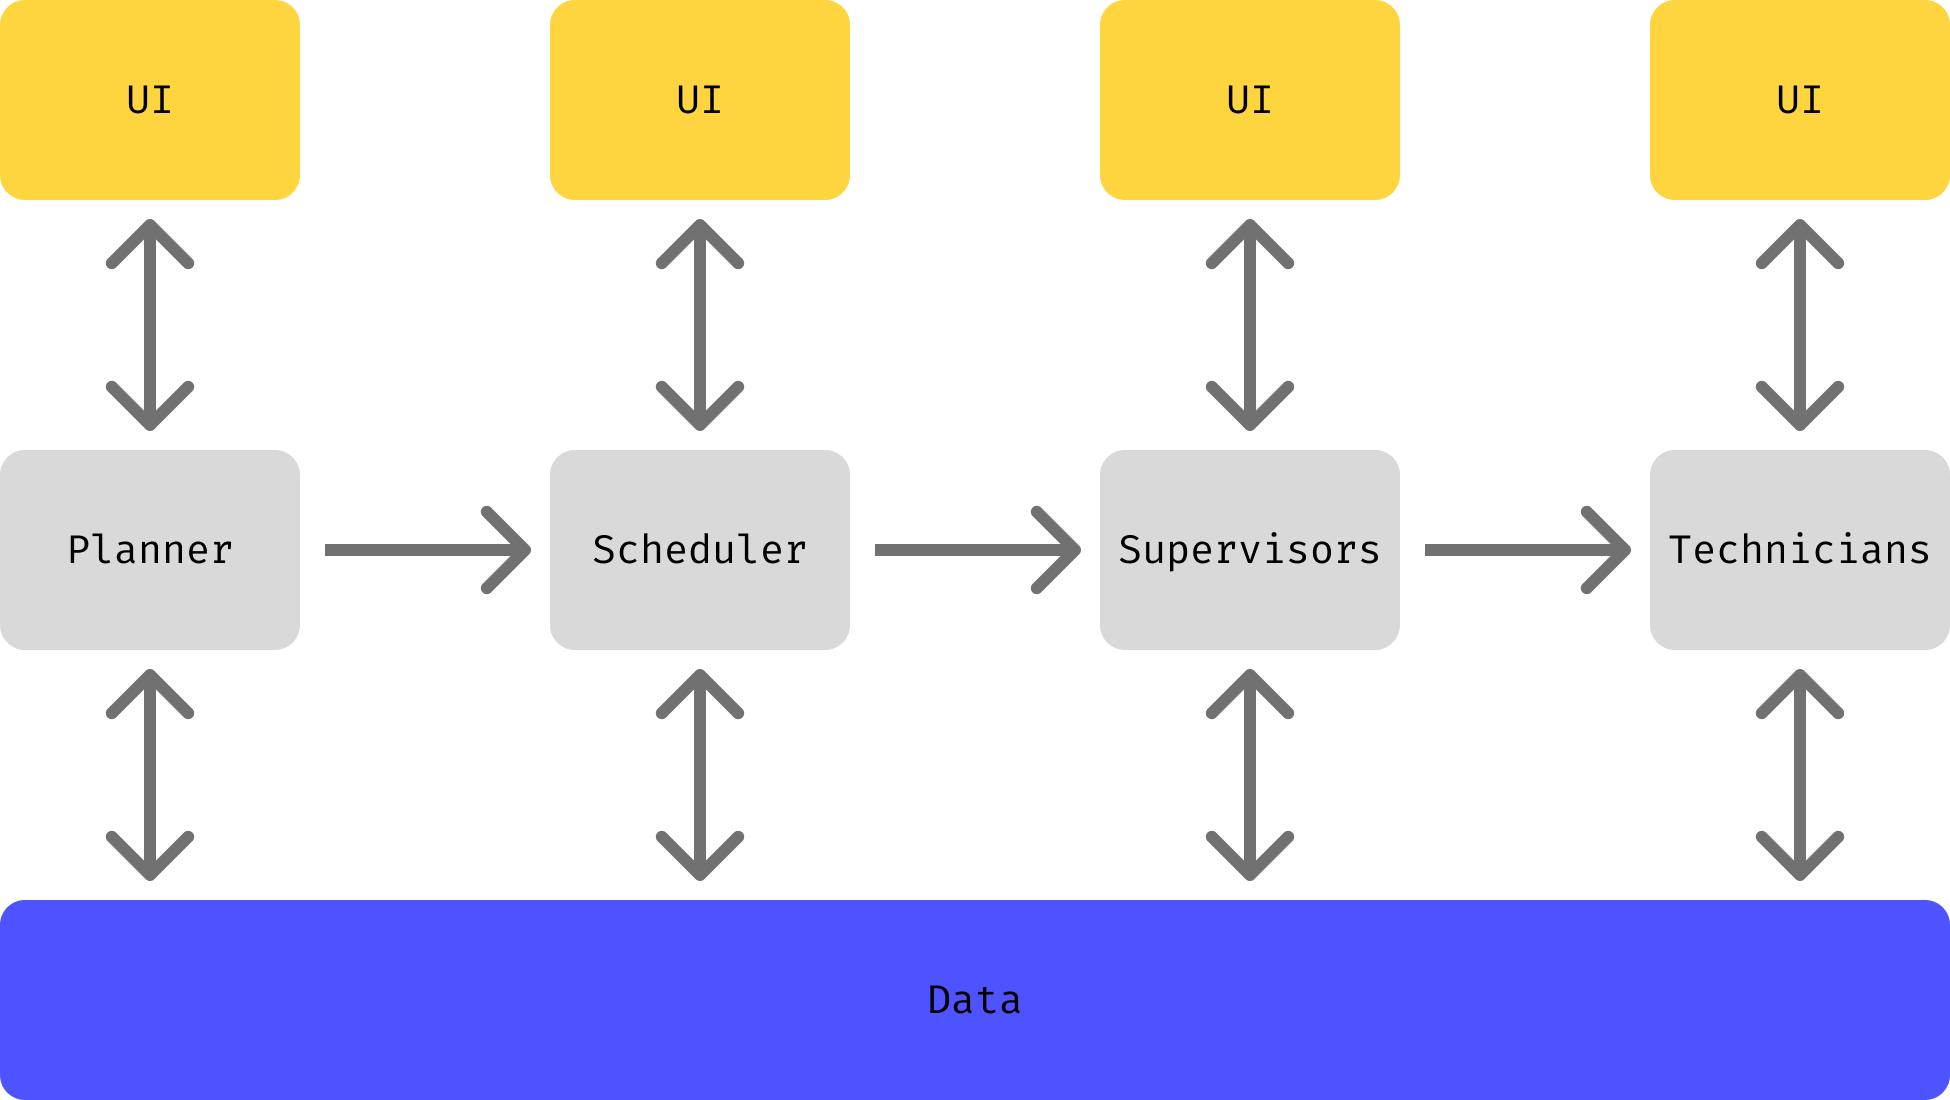
\includegraphics[width=1.0\textwidth]{figures/Scheduling Process Integrated.png}
\label{fig:integrated:maintenance-process}
\caption{Overview of the scheduling process when modelled as actors. When LNS is encapsulated 
is an actor it becomes possible to optimize parts of a large process individually instead of 
optimizing the scheduling problem globally from a single model inplementation.}
\end{figure}


\subsection{Continuous Optimization}
With actor-based metaheuristics it becomes simple to extend a metaheuristic to run
indefinitely with it being able to optimize based on the latest best 
available information. This may seem like a minor detail as you could argue that you should only ever optimize the schedule when there is 
an explicit need for it, but consider the case when you start adding more than two actor to a scheduling system, then there arises a need
to coordinate people in time as each will have to run their optimizer on after another.

\bibliography{refs}

\bibliographystyle{elsarticle-harv}
\end{document}

hello
\endinput
